% !TEX root = pfe-book4.tex
%!TEX TS-program = pdflatex
%!TEX encoding = UTF-8 Unicode


\cleardoublepage
%\mainmatter
\chapter{Optical Instruments}
\label{ch-02}

\section{The Prism}
The armamentarium of instruments employed in labor­atories and industry have such a big turnover that if a scientific worker dropped out of research for a decade or two he would have to start studying all over again. But today and, most likely, in the distant future he will again meet his old acquaintances, the prism and the lens. Let us recall the simple laws that light obeys in interactions with these transparent materials. Incidental­ly, transparency is a relative notion. For certain electromagnetic waves, even wood and concrete are transparent.

The laws of interaction of a light ray and a body ca­pable of reflecting and refracting the ray are simple until the wave aspect of the light waves becomes involved. These are the \emph{law of reflection} (the angle of incidence is equal to the angle of reflection) and the \emph{law of refraction} of light (\figr{fig-2.1}). It will be recalled that when a light ray falls on the boundary between two media, it is deflected from its recti­linear path. The angles of incidence $i$ and of refraction $r$ are connected by the relation
\begin{equation*}%
n = \frac{\sin i}{\sin r}
\end{equation*}
This law was established, in very careful measurements, by the Dutch physicist Willebrod Snellius or Snell (1591- 1626), professor at the University of Leiden. The contents of his course of lectures in which he described the phenomena of light interacting with transparent bodies was well known to a small (in those days) circle of European scholars.

\begin{figure}[!ht]
\centering
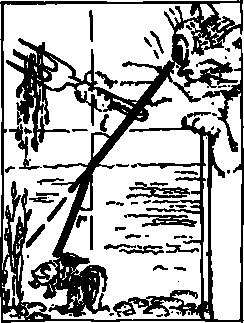
\includegraphics[width=0.4\textwidth]{figures/fig-02-01.pdf}
\caption{The law of refraction.}
\label{fig-2.1}
\end{figure}

That most likely was the reason Ren\'e Descartes’ (1596-1650) article entitled \emph{Discours de la M\'ethode} (1637) was scoffed at by his contemporaries, for it was here that Descartes would appear to have ``proved'' this law with the aid of rather strange reasoning. Descartes’ nebu­lous verbiage did not excite the admiration of his colleagues. But the fact that his discourse did indeed result in the correct formula was explained away very simply: he was said to have fitted arguments to a result that had already been obtained. And so Descartes had also to experience accusations of plagiarism.

Perhaps, after all, we might join the sceptical attitude of his contemporaries. Descartes considers a ball thrown onto a weak net. The ball breaks through the net and loses half its speed. Then, writes the great philosopher, the motion of the ball differs radically from its original design, in one direction or another. It is indeed hard to get at what the real meaning is. Perhaps Descartes wanted to say that the horizontal component of velocity of the ball does not change while the vertical component does, for it is precisely in that direction that the net obstructs the motion of the ball.

But let us get back to the law of refraction.

The angles $i$ and $r$ are ordinarily laid off from the position of the normal as shown in \figr{fig-2.1}. The quan­tity $n$, which is called the index of refraction (or refrac­tive index), depends on the media involved. In order to compare bodies as to optical properties, it is convenient to set up a table of the indexes of refraction for the case of an incident ray from the air (or, if one is a pedant, from a vacuum) into a medium. In this case, the angle of refraction is always less than the angle of incidence, and hence the refractive index is greater than unity.

The refractive index grows with the density of the medium. For diamond, it is 2.4 and, for ice, it is 1.3. 

I'm not going to give a table of refractive indexes, but if I did, I’d have to indicate for what wavelength of light the data are given. The index of refraction depends on the wavelength. This is an important phenomenon underlying operation of a number of instruments that resolve electromagnetic radiation into a spectrum and is called dispersion.

If light falls from one medium into a medium of smaller density, then a complete internal reflection can occur. In this case, the refractive index is less than unity. As the angle of incidence increases, the angle of refraction will approach \ang{90}. Provided that $\sin r = 1,\, \sin i = n$ the light will cease to pass into the second medium and will be reflected \emph{in toto} at the interface. For water, the angle of total internal reflection is equal to \ang{49}.

The refraction of light by means of a plane plate can be used to shift a ray to a position parallel to itself. And with the aid of a prism a light ray can even be turned around.

If the reader wants to recall the derivation of the for­mula for the angle of rotation $D$ of a light ray, he can find it in a school textbook. The derivation only requires a few facts from elementary geometry, but it is very un­wieldy, particularly if it is done for a thick prism and for an arbitrary value of the angle of incidence of the ray on the prism. A simple formula is obtained if the prism is thin, and the angle of incidence of the ray on the face of the prism does not differ greatly from a right angle. If that is the case, then
\begin{equation*}%
D = (n-1) p
\end{equation*}
where $p$ is the angle between the faces of the prism. Using a prism, the great Newton demonstrated for the first time (this was at the end of the seventeenth century) that white light is not monochromatic but consists of rays
of different colours. Violet rays undergo the greatest de­flection, and red the smallest. That is precisely why we say ultraviolet and infrared rays, and not infraviolet and ultrared.

The scientific world learned of Newton’s discovery in 1672. In explaining his experiments, Newton is clear and exact. Therein lies his genius. As for his discussions of the matter, it is no easy job to plough through them. Only after much digging in the verbiage can one gather that although the author had promised to depict facts and not to create hypotheses (Newton’s famous phrase: \emph{``hypothesis non fingo''}, or ``I do not frame hypotheses'') he did not carry out his promise. Many of the axioms and defini­tions, like, say, ``a ray of light is its minutest part'' are very strange indeed to the modern ear.

In chemistry the spectrograph still reigns supreme, and the main component is Newton’s prism. The material must possess a high degree of dispersion. Prisms for spec­trographs are made out of quartz, fluorite, and rock salt. The light to be resolved is passed through a slit located in the principal focal plane of the input lens. That is why a parallel beam of light falls on the prism. Photons of different frequency go in different directions. The sec­ond, or exit, lens collects identical photons into a single point of the focal plane. The spectrum may be viewed with the naked eye, but then a piece of frosted glass is required. The spectrum can also be photographed.

At the present time, spectra are registered by automatic recorders. An energy receiver in the form of a photocell or thermocouple slides along the spectrum. The receiver generates a current whose strength is proportional to the light intensity. This current deflects the moving part of the recorder in exactly the same way that the current of a galvanometer deflects the needle. The deflected part has an attached stylus that records the spectrum on a roll of paper tape that unwinds at a constant rate.

\section{The Lens}

A whole industry is engaged in the manufacture of lenses. These are transparent bodies bounded by two spher­ical surfaces or one spherical surface and one plane surface, and they come in all imaginable sizes. Some devices use lenses the size of a small coin, in others (large tele­scopes) there are lenses several metres across. The manu­facturing of large lenses is a real art, because a good lens must be homogeneous throughout.


Every reader knows what a lens is and probably knows the main properties of one. A lens magnifies, a lens can focus rays of light. Using a lens placed in a strong beam of light (from the sun), it is easy to set a piece of paper afire. A lens ``collects'' rays of light in a single point, the focus (focal point) of the lens.

The fact that parallel rays converge to a single point and, conversely, that a lens produces a parallel beam of rays if a point source of light is placed in the focus of the lens can be demonstrated with the aid of the law of refraction and simple geometric reasoning.

If a point does not lie in the focus but at a distance $a$ from the centre of the lens, then rays emanating from it collect at a distance $a'$. These two distances are con­nected by the familiar formula
\begin{equation*}%
\frac{1}{a} + \frac{1}{a'} = \frac{1}{f}  
\end{equation*}
where $f$ is the focal length of the lens. It is easy to show that light rays proceeding from an object twice the focal length produce an inverted and reduced (in the ratio of $a'/a$) image between the focus and the double focal length.

If the object is placed in the position occupied by the image, then the image takes up the position occupied by the object. This is the so-called \emph{principle of reversibility of light rays.}

When we use a lens to magnify, the object lies between the lens and its focal point. In this case the image is not inverted and lies on the same side as the object (\figr{fig-2.2}).

The difference between the case of a magnifying glass and the two preceding instances is this: a magnifying glass produces virtual image, whereas in other positions of the object we obtain images that can be seen on a screen or photographed. We can justly call them real.

The magnifying power of a magnifying glass is the greater the smaller its focal length. The limiting possibil­ities of a magnifying glass are rather modest: the angle of view at which the virtual image is visible can only be magnified 20 to 30 times the angle of view at which we see the object with the naked eye.

\begin{figure}[!ht]
\centering
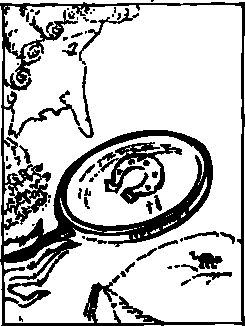
\includegraphics[width=0.4\textwidth]{figures/fig-02-02.pdf}
\caption{The magnification by a lens.}
\label{fig-2.2}
\end{figure}


Many optical instruments would be simple in the ex­treme and would consist of single lenses if it were not for a number of unavoidable defects. We want a parallel beam of white light to be focussed by a lens to a single point. But dispersion hampers this. Photons of different colour are deflected by the lens in different directions.

As a result, instead of a point we obtain a coloured line spread out along the axis of the lens. This is known as \emph{chromatic aberration}.

Another bit of trouble is \emph{spherical aberration}. The rays that are closer to the axis of the lens will come to a focus at a more distant point than rays whose paths lie farther away from the axis.

Also, the behaviour of rays falling on the surface of the lens at large and small angles is quite different. In­ stead of a point we obtain a glowing nucleus displaced away from the proper position. A tail-like appendage is attached to the nucleus. This effect is termed a \emph{coma}. The word ``coma'' translated from the Greek is something in the nature of ``loose hair''.

And this is not the end of the list of distortions that plague the single lens. When we examine a square, we see a quadrangle with the vertices in the form of arcs convex inwards. This is because the rays emanating from the vertices of the square and from the midpoints of its sides are refracted in different ways.

Another defect of a lens that plagues designers of opti­cal instruments is termed as \emph{astigmatism}. If a point lies a good distance from the principal optical axis of the lens, then its image splits into two strips perpendicular to each other and displaced in opposite directions with re­spect to the position of the ideal image.

And there are still other distortions. Specialists in lens production classify all types of distortions into seven basic types. We have mentioned only five.

As so often is the case in technology, making a good lens amounts to a compromise. It is quite clear that increasing the size of a lens increases the distortions, but, on the other hand, the illumination of the image (that is, the number of photons of visible light per unit area) is proportional to the square of the diameter of the lens (that is, its area). But this is not all. Suppose the object depicted by the lens is at a considerable dis­tance. Then the image will come to a focus. The smaller the focal length the smaller the dimensions of the image. In other words, the light flux emanating from the object collects over a smaller area. Thus, the illumination is inversely proportional to the focal length.

For these two reasons, the square of the ratio of the diameter of a lens to its focal length is called the \emph{aperture ratio} of the lens.

Thick lenses have the smallest focal lengths. These are lenses whose surfaces are formed by small radii. But these are precisely the lenses that produce the greatest distor­tions. This means that increasing the aperture ratio of a lens (whether done at the expense of its dimensions or the radius of curvature) leads to a worsening of the image. This is no easy task that confronts engineers and design­ers.

\section{The Camera}
In its simplest form, a \emph{camera} is a lens that plays the role of a window in a dark box. The image produced by the lens is recorded on a photographic plate located opposite the window.

Now, a simple lens distorts any image. For this reason, it is replaced by a set of lenses designed to eliminate the optical defects encountered. The set of lenses is termed a photographic lens.

The question now is how to get around the distortions we have mentioned. Quite some time ago the idea was suggested to use a system of lenses chosen so that the defects of each one are eliminated by the defects of the others. This principle of obtaining a plus by multiplying two minuses has proved to be sufficient to eliminate all seven defects with the aid of only three lenses. That is the principle. Actually to obtain the most perfect images requires still more complicated combinations. One such combination (though by far not the most complicated) is depicted in \figr{fig-2.3}.
This system of concave and convex lenses is capable of producing a nondistorted image under appreciable variations of the degree of magnification. The first and third components of the system are capable of moving with respect to each other, thus attaining a continuous variable three-fold focal length. 
\begin{figure}[!ht]
\centering
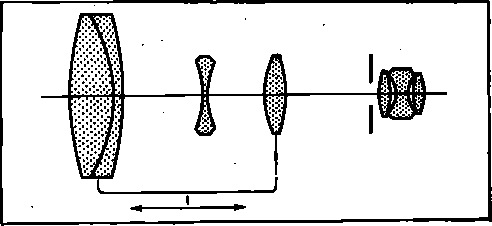
\includegraphics[width=\textwidth]{figures/fig-02-03.pdf}
\caption{A compound lens.}
\label{fig-2.3}
\end{figure}


A camera requires a rather simple device to ``focus'' it. This means making it possible to vary the distance between the centre of the lens and the film. Occasionally one sees old cameras in the form of an accordion that can be squeezed together. And I must say that such came­ras do a fairly decent job.

In a modern camera that fits into the palm of your hand, this operation is performed more neatly: just a tiny spiral turn of the lens mount. As is evident from our discussion of the aperture ratio of a lens, the quality of the image improves if we diminish the eye of the camera as much as possible. This is done with the aid of a dia­phragm of variable diameter.

We choose the dimensions so that it is as small as possible but lets in sufficient light to produce a good im­age for the specified exposure.

Did you ever think of why the old photographs taken when photography was in its infancy look so stilted, so tense? The explanation is simple: the photographer had to resort to long exposures and that is why he ex­horted his client not to move: ``Hold it, \ldots{}''

The fight to get a good image at minimal exposure is carried out along two lines. The first is to perfect the pho­tographic lens. This is done not only by suitable selection of the geometry of the lenses that make up the compound lens. In a compound lens  nearly half the light is reflected. First, this results in a loss of illumination of the image, second, it produces a light background that reduces the degree of contrast of the image. This is combatted by a technique called \emph{lens coating}. The surface of each lens is covered with a very thin film. Due to the phenomenon of interference, the portion of reflected light is drastically reduced. Compound systems with coated lenses can be recognized at once: the glass has a bluish tinge.

Another way to improve photographs is to perfect the film.

A few words are in order concerning the photochemical process that leads to the formation of an image. The photosensitive layer is a gelatin with embedded crystals of silver bromide and a small admixture of silver iodide. The size of the crystal grains ranges from a thousandth to a ten-thousandth of a millimetre. The number of grains per square centimetre of film is anywhere from ten thou­sand to hundreds of thousands. Under the microscope, the layer of photographic emulsion reveals that the grains are rather close together.

Photons falling on a grain of emulsion disrupt the bonds between the atoms of silver and the atoms of the halide. The number of atoms of silver that are released is strictly proportional to the number of photons incident on the film. The photographer chooses an exposure time during which a considerable number of bonds between the atoms of silver and bromine are disrupted. And yet the exposure should not be too long. That would result in a complete destruction of the bonds between atoms of silver and bromine in all crystals. When the film is developed, the crystals release all the silver they contained and the film is black throughout.

If the exposure is correct, the photographic plate will reveal the latent image of the object. In each grain, the number of disrupted bonds is proportional to the number of photons incident on the grain. The process of devel­oping the film consists in permitting the potentially free atoms of silver to combine. Then the amount of released silver on the negative after developing the film will be proportional to the intensity of the light.

From the foregoing it is probably evident to the reader that the smallest details revealed by a photograph of an object cannot be larger than the size of a grain crystal of silver bromide.

After the film is developed the next stage is to fix it. The fixing process consists in removing the undecomposed silver bromide. If these grains are not removed, then the film is spoiled when exposed to light because the grains release all the silver they contain.

The physics of obtaining a positive image is so obvious that we will not dwell on it.

The technology of modern coloured photography is not at all simple and merits our full admiration, yet the physics of that process, on the contrary, is very simple indeed. The model of our perception of colour that was proposed in the middle of the eighteenth century is quite true. The human eye has receptors of three colours: red, green, and blue. By combining these colours in different combinations, we obtain a perception of any colour. Accordingly, to obtain a coloured image we need a three-layer film. The upper layer is sensitive to blue rays, the middle layer to green, and the bottom layer to red. We will not go into how chemists achieve this. The coloured negative is transformed into a coloured positive, again through the use of three-layer photographic paper.

\section{The Eye}

The eye created by nature is marvelous physical in­strument. The possibilities of distinguishing tens of thousands of shades of colour, of seeing close to and far away, of perceiving, via two eyes, the spatial relationships of objects, of being sensitive to extremely slight light in­ tensities are all properties that place the human eye in the category of the highest-quality instrument. True, the human eye sees only a small portion of the spectrum.

The eyes of some animals, however, overcome this defect to a certain extent.

In some ways, the eye is reminescent of the ordinary camera. The role of the camera lens is played by the crystalline lens, which is double-convex. The crystalline lens of the eye is soft and capable of changing its shape under the action of muscles that embrace it. Therein lies the process of accommodation of the eye that permits it to see with equal ease both nearby and distant objects. With age, the crystalline lens becomes hard and the muscles weaken, and then glasses (spectacles) are needed for distance and reading.

The image of an object is projected onto the rear wall of the eye, and the optic nerve transmits this perception to the brain.

The normal eye of a young person is capable of discerning the details of an object located at a distance not less than 10 centimetres. Ordinarily, with age comes farsight­edness, and that distance increases to 30 centimetres.

In front of the crystalline lens is the pupil, which plays the role of the diaphragm of the camera. The human pupil can vary in size from 1.8 to 10 millimetres.

The role of the photographic plate on which the image is formed is played in the human eye by the retina, which has a very complicated structure. Under the retina lies the optic epithelium, which consists of light-sensitive cells called rods and cones. You can compare the number of these cells to the number of grains of silver bromide in the photographic plate. There are over a hundred million optic cells in the human eye. Since the normal person is capable of distinguishing colours, it is clear that the optic cells possess differing sensitivity to different portions of the spectrum. We arrive at the same result if we assume that the cells are divided into classes recep­tive to different portions of the spectrum.

If vision is normal, the rear focus of the eye in the calm state lies on the retina. If it lies in front of the retina, the person is \emph{nearsighted}; if it is behind the retina, the person is \emph{farsighted}. These two most common defects of sight are due to an excessively thick or thin crystalline lens. Some people also suffer from \emph{astigmatism}. In this case, the crystalline lens in the normal state does not have a correct shape bounded by two spherical surfaces.

All these defects can be rectified by eye glasses, which, together with the crystalline lens, yield an optical system that can focus the image of a distant object on the retina.

The lenses of spectacles are characterized by what is called \emph{diopter} (a unit of the power of lenses). The optic power of a lens is inversely proportional to the focal length. The optic power in diopters is equal to unity divided by the focal length in metres. The focal lengths of dispersing lenses that nearsighted people use in their eye glasses are negative.

The angle of vision of the eye is much greater than appears to us. A number of events that occur at right angles (\ang{90}) to either side of our straightforward view are recorded directly by our subconscious. This fact leads some people to the erroneous idea that they ``feel'' some­ one is looking at them, without actually seeing the person.

The eye poorly perceives objects seen at an angle of less than one minute of arc, even if the illumination is very good.

\section{Polarizers}

A light wave is an electromagnetic wave. As was men­tioned in the third book of this series, pictorial experi­ments have demonstrated that the vector of the electric field is perpendicular to the direction of motion of a ray of light. If this fact is interpreted from the standpoint of light being corpuscular (in the form of particles), then we must say that a particle of light -- the photon -- is not a sphere but an arrow. In a number of complicated cal­culations, theoretical physicists have come to the con­clusion that the photon possesses spin (equal to 1). Thus, the concept of a photon as an arrow is quite natural.


The ordinary ray of light is a stream of photons whose spins are perpendicular to the direction of propagation of the light but are distributed uniformly in the form of a circle perpendicular to the light ray. This type of light ray is said to be \emph{non-polarized}. However, in a number of cases we have to do with a beam of photons in which all the spins are in one direction, or, to put it differently, we have to do with electromagnetic waves, the electric vectors of which have a very definite direction. Such rays are said to be \emph{polarized}.

One way to obtain polarized rays consists in making the light ray pass through a low-symmetric crystal. Such crystals, when suitably oriented with respect to an inci­dent light ray, possess the capability of splitting the natural ray into two rays polarized in two mutually perpendicular directions.

Unfortunately, I cannot give the reader even a rough idea about how this happens because the molecules of a crystal ``receive'' waves with differently arranged electric vectors in different ways. I can see that the preceding sentence hasn’t helped matters much. But I can at least assure the reader that the theory of the splitting of light rays exists and it is a very good theory that is capable of describing all the fine details of this exciting phenom­enon. For instance, it is possible to predict how the passage of light will change if we place the crystal at different angles to the ray of light.

By splitting a non-polarized ray into two polarized rays, we can then easily make one of the rays go off in some desirable direction. The result will be what is called a \emph{Nicol prism}, named after the Scottish physicist William
Nicol (1768-1851). The instrument was made in 1828. It is interesting to note that in those days all explana­tions of the polarization of light were given in the language of particles and it was considered an excellent confirmation of the corpuscular theory of light proposed by Newton.

Soon afterwards the interference and diffraction of light were discovered, and these were so naturally accounted for in terms of waves that the theory of particles of light was buried. But a century passed and the theory was resurrected, like the phoenix arisen from ashes. True, this time merely in the modest attire of one of two as­pects of the electromagnetic field.

If a polarizer is placed in the path of the light, the intensity of the ray falls off, as is to be expected, by a factor of two. But the most interesting phenomenon, which is what proves the existence of polarization, occurs when we place a second instrument in the path of the light ray. This instrument is called an \emph{analyzer}, although it does not at all differ from the first Nicol prism. Now let us turn the Nicol prism about the light ray. It turns out that for a certain mutual position of the two prisms, the intensity of the light that has passed through both Nicol prisms remains the same as it was in the absence of prisms. We then say that the Nicol prisms are parallel in that position. Now start turning the analyzer. When we have turned it through \ang{90}, the light ceases to come through. We then say the Nicol prisms are crossed.

In an intermediate position when the second Nicol prism is turned from the parallel position through an angle $\alpha$, the intensity is equal to $1/2 \cos^{2} \alpha$. The formula is readily explainable if we assume that the vector of the electric field has been divided into two components, one perpendicular and the other parallel to the ``slit'' of the analyzer. Now the intensity is proportional to the square of the amplitude of the wave, that is, to the square of the electric vector. That is why variation in light intensity must occur in accord with the law of the square of the cosine.

Such an analysis of polarized light has a number of practical applications. Suppose the Nicol prisms are crossed and a transparent body that is capable of turning the electric vector of the wave is interposed between them. We then have field brightening. Charged bodies have this capability. Depending on the amount of voltage, the rotation of the light vector and, together with it, field brightening beyond the crossed Nicol prisms will be different. We will see pretty patterns, and coloured too, because photons of different colours behave differ­ently. These patterns permit judging the voltages in the sample or deciding whether the molecules that make up the sample are oriented or not. This is important information, and so a good microscope is equipped with two Nicol prisms so that the image of an object can be seen in polarized light. The information about the struc­ture is then much richer.

Solutions of many substances (for example, sugar solu­tions) have a certain rotatory power that permits turning the electric vector of a light wave. Here, the angle of rotation turns out to be strictly proportional to the amount of sugar in the solution. We can thus adapt a polarimeter for measuring sugar content. Such instruments are termed saccharimeters and can be found in any chemical laboratory.

These two examples do not exhaust the use of polarimeters but they are probably the main ones.

\section{The Microscope and the Telescope}

The optical part of a \emph{microscope} consists of an eyepiece and an objective. The eyepiece (or ocular) is the lens to which the eye is applied; the objective is dose to the object being studied. The object is placed at a distance somewhat greater than the focal length of the objective. The image obtained between the objective and the eye­ piece is inverted. It is necessary that it appear between the eyepiece and the focus of the eyepiece. The eyepiece plays the role of a magnifying glass. It can be demonstrat­ed that the magnifying power of a microscope is equal to the product of the magnifications of the eyepiece and objective taken separately.

At first glance it might appear that a microscope can be used to discern arbitrarily small details of an object. For example, why not make a photograph by increasing the dimensions thousands of times, then examine it in a microscope and obtain a million-fold magnification, and so on.

This kind of argument is totally fallacious. First of all, let us recall that increasing the size of photographic pictures is limited by the size of the grains of the film. The point is that each tiny crystal of silver bromide acts as a whole. The reader most likely has seen highly mag­nified photographs and has noticed that the magnifica­tion does not at all improve the details of the picture but only smears them out.

But if we discard the operation of photography and magnify the image optically, and this is possible merely by increasing the number of lenses, we will soon see that any great magnification is meaningless. The useful mag­nification of any instrument is limited by the wave aspect of the electromagnetic field. Whether we are examining an object through a magnifying glass with the naked eye or with the aid of a microscope or telescope, in all cases the light wave proceeding from the glowing point must pass through an opening. But in that case we have to deal with the phenomenon of \emph{diffraction},\label{diff-ref} that is, the deviation of the light ray from its rectilinear path. To one degree or another, the ray ``peeks around the corner'' and so the image of the point is never a point but a spot. And no matter how you try, it is impossible to make the size of the spot less than the wavelength of the light.

It is essential to be able to estimate under what condi­tions the path of the electromagnetic wave departs appre­ciably from the rectilinear path.

If $x$ is the linear deviation from the rectilinear path observed at a distance $f$ from the source of radiation, and the size of the obstacle (or aperture) in the path of the ray is equal to $a$, then we have the following rela­tionship:
\begin{equation*}%
x = \frac{\lambda f}{a}
\end{equation*}
Here, $\lambda$ is the wavelength. From this equation it follows that diffraction can be observed both in the case of mi­nute particles and celestial bodies. The whole point is the wavelength and the distances we are dealing with. The same goes for apertures as well. Diffraction is not only observed in the case of minute openings. For exam­ple, an opening the size of a tennis ball permits observing diffraction phenomena; true, only at distances of the order of hundreds of metres.

The simple equation we wrote down enables us to gauge the limiting possibilities of microscopes and telescopes. A microscope does not permit us to see features of an object smaller than a micrometre. Now millimetre sizes can be seen with the naked eye. This means that optical microscopes should not be used to seek magnifications
greater than 1000.

This restriction has to do with optical microscopes only. Now if it were possible to design a microscope oper­ating not with light rays but with some other rays with smaller wavelengths, then the useful magnifying power of the microscope could be increased. Just such a microscope exists and can be found in many scientific laboratories. It is called an \emph{electron microscope}. The wavelengths of electrons can be made very small (see page \pageref{de-broglie-equation}). Electron microscopes can resolve structural details of the order of ten millionths of a millimetre.
\begin{figure}[!ht]
\centering
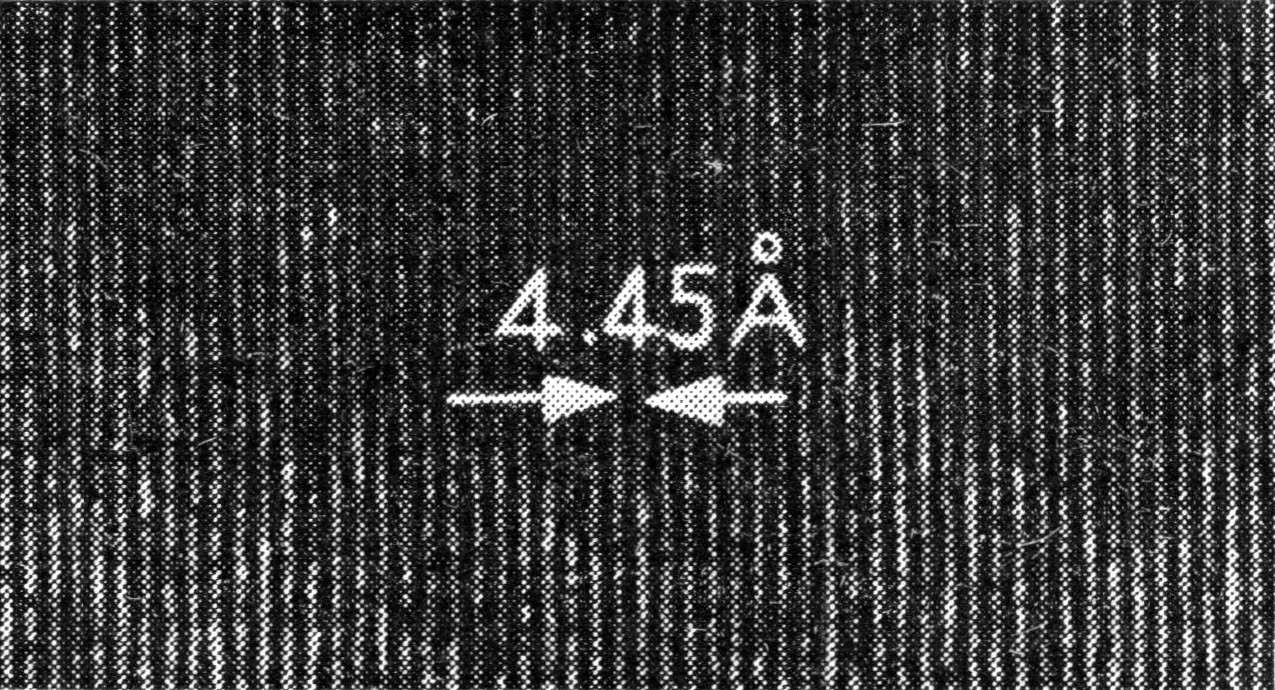
\includegraphics[width=0.4\textwidth]{figures/fig-02-04.jpg}
\caption{A compound lens.}
\label{fig-2.4}
\end{figure}

Biologists have seen molecules of DNA, the long molecules that carry hereditary characteristics from parents to progeny. Protein molecules have been observed, also the structure of cell membranes and details in the structure of muscle fibres. The photograph in \figr{fig-2.4} is a record: this is a 3-million-fold magnification of the crystal lattice of the mineral pyrophyllite showing the distance between the planes of the crystal at 4.45 ang­stroms!

The limit of the electron microscope has to do not with its resolving power (we can easily reduce the wavelengths of electrons) but with the contrast in the image: the molecule under investigation has to be backed: placed on a base (backing), which itself consists of molecules. On the background of molecules of the backing, it is difficult to discern the molecule of interest.

An electron microscope is a complex and very expensive instrument about a metre and a half in height. Electrons are accelerated by a high voltage. The principle of magnification is the same as in the optical microscope. It is produced by lenses. But, naturally, they are not at all like those of an ordinary microscope. The electrons are focussed with the aid of electric fields of high-voltage metallic plates with apertures and by means of coils that set up a magnetic field.

There are a great variety of techniques that help to produce the image. Microtomes are used to obtain ex­tremely thin sections for transillumination, the molecules on the backing are tinged by depositing metallic vapour on them. It is also possible to obtain a replica of the speci­men, that is, by coating it with an extremely thin film of transparent material and then etching out the object itself.

Electron microscopy is a big and important division of physics well deserving of a separate chapter, but the size of this book presses me onwards.

Our next topic is the \emph{telescope}. As early as the 16th century suggestions were made that distant objects could be examined with the aid of convex glasses. Yet I think that the real invention of the telescope (actually a spyglass) was made by the great Galileo. He constructed it in July 1609 and a year later published his first obser­vations of the night sky.

Like the microscope, a telescope (\emph{refracting telescope}, to be exact) is in principle a combination of two lenses: the objective, that forms an image from a distant object, and the eyepiece. Since an infinitely distant object is viewed, its image is created in the focal plane of the objec­tive. The focal plane of the eyepiece coincides with the plane of the objective, and beams of parallel rays emerge from the eyepiece.

The power of the telescope increases with the diameter of the objective. For example, a \SI{10}{\centi\meter} diameter telescope permits viewing features on Mars about \SI{5}{\kilo\meter} in size. With a \SI{5}{\meter} diameter telescope, objects up to \SI{100}{\meter} across can be resolved on Mars.

Astronomical observatories are equipped not only with refracting telescopes but also \emph{reflecting telescopes}. Since our aim is the study of distant objects and it is required to gather the light rays into a focus, this can be done by means of a spherical mirror as well as a spherical lens. The obvious advantage in this case (a mirror) is that we get rid of the chromatic aberration. The defects of the mirror telescope are connected only with the difficulty of making high-quality mirrors.

Quite naturally, the telescope too has a limit to the useful magnifying power it is capable of producing. This limit is associated with the wave nature of light. A ray of light from a distant star spreads out into a circle and this places a limit on the angular distance between stars that we are able to resolve in the telescope. Again, the desire to increase the power of the telescope is linked up with increasing the diameter of the glass. The limiting possibilities of the telescope probably lie somewhere close to one tenth of a second of arc.

During recent years, new instruments have appeared and are helping astronomers study the stars in all portions of the spectrum of electromagnetic waves coming to us from outer space. We will come back to this topic again in the seventh chapter.


\section{Interferometers}

As we have already pointed out a number of times, the electromagnetic field possesses a wave aspect. And so also do beams of particles -- electrons, neutrons, protons. Sound is the result of mechanical displacements of the medium and these occur in accord with the wave law. Common to all these physical processes is the possibility of ascribing to any radiation a wavelength, frequency, and rate of propagation; these are connected by the equa­tion $c = \lambda \nu$. The simplest kind of radiation is monochro­matic, that is, it is described by a single wavelength. In the general case, radiation constitutes a complex spectrum, that is, a sum of waves of different wavelength and intensity.

The wave aspect of radiations is revealed in the combin­ing of waves and also in scattering due to bodies in the path of the rays. An important special case of wave scattering is diffraction. The composition of waves is \emph{interference}.

Here we will deal with the interference of light. This phenomenon underlies the operation of a number of in­struments used for measuring distances and also certain other physical quantities. Instruments that use the phe­nomenon of interference for applied purposes are called \emph{interferometers}.

The principle for measuring distance consists in cal­culating the number of waves that fit into the distance being measured.

This might appear to be a simple thing to do. Take two sources of light and bring both beams to a single point. Then depending on whether the waves arrive at the point of observation ``hump to hump'' or ``hump to dip'', we get a bright or a dark spot. Now let us pose the problem of measuring the distance over which we wish to move one of the light sources. This motion will cause the phase rela­tionships of the two waves at the point of observation to change. All we have to do is calculate the number of alter­nations of light and darkness and then, taking into account the geometry of the experiment and knowing the wave­length of the light, readily compute the amount of dis­placement.

In principle that is correct. But acting in this fashion we will not observe a pattern of alternating light and darkness. The screen will remain light all the time and so this simple experiment is a failure.

What is definitely known is that if two rays of light emitted by two different sources come to a point, they will always reinforce each other. Then perhaps the wave theory is fallacious?

No, the theory is correct and electromagnetic radiation has a wave aspect. But we began with an erroneous supposition. For interference to be observed, it is neces­sary that an invariable phase difference obtain all the time between the waves being combined. But phase re­lationships even between waves emanating from two atoms of one and the same source are quite accidental. We have already mentioned the fact that atoms throw out photons without ``agreeing'' among themselves on their behaviour. Thus, two different sources radiate haphazardly; this is called \emph{incoherent radiation}.

But then coherent radiation must be something in the nature of a dream. We shall now see that that is not so. 

The solution is extremely beautiful and at the same time simplicity itself, like most original concepts: the problem is to make the radiation of the atom combine with itself. And to do that it is required to split the ray coming from each source into two parts and make the two parts of the single ray traverse different paths, and finally bring them together. Then, under such conditions while observing interference and changing the differences in the paths of the parts of the split ray, we can indeed measure the displacement and length by computing the number of alternations of light and darkness.

What we have just described is the principle underlying interferometer measurements that was discovered in 1815 by the French physicist Augustin Jean Fresnel (1788-1827). Let us now consider the methods underlying the action of interferometers by means of which one can split a ray of light and create different paths between the split
portions of the ray.

Now let us dwell in more detail on the interference of
light rays reflected from the inner and outer sides of a transparent plate or film. This is of interest both because of its practical utility and because it is observed in nature. Besides, this is a good example for illustrating many
important concepts that we use in describing light waves and other electromagnetic waves.

\begin{figure}[!ht]
\centering
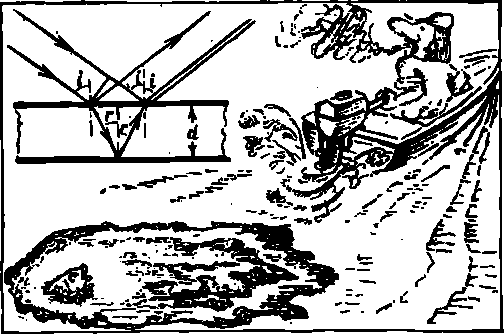
\includegraphics[width=\textwidth]{figures/fig-02-05.pdf}
\caption{An interferometer.}
\label{fig-2.5}
\end{figure}

\figr{fig-2.5} enables us to compute the phase shift be­ tween two such rays. The difference in phase is determined by the difference in routes, that is, the difference in the paths taken by the two rays. From the drawing it is evi­dent that the path difference is $x=2 d \cos r$. But then there is the question of how to proceed from the path difference of the rays to the phase difference, which is what determines whether the two waves will reinforce or weaken each other.

If the reader is not afraid of the cosine formula, we can discuss this matter. The oscillation of a light vector at any point in space can be written down as follows: $A \cos 2 \pi \nu t$. The phase shift through the angle $\varphi$ signifies the necessity of adding this angle to the argument of the cosine. If we want to compare the phases of points of one and the same wave, which points are separated by a distance $x$, we have to take into account the number of wavelengths that fit into that interval and then multiply the result by $2 \pi$. That quantity is the \emph{phase shift}. Thus,
$\varphi =2 \pi x/\lambda$.

Now let us return to the interference of rays in the plate. We have written down the difference in paths. All that is left, then, is to divide that quantity by $\lambda$. But wait a minute. Is the wavelength of light in a vacuum the same as inside a transparent plate? Something makes us suspect that when a wave of light passes from one medium into another it undergoes a change. We know about \emph{dispersion} -- when photons of different frequency behave differently. The frequency, wavelength, and rate of propagation are related as follows: $c=\nu \lambda$. Which of these quantities undergoes a change when the wave enters a new medium? Experiment can tell us. We can measure the rate of propagation of the wave directly in the body and then see that the refractive index, which makes the wave alter its direction of motion when falling obliquely on the interface between the two media, is equal to the ratio of the rates of propagation of light in the media. If one of the media is air (a vacuum, to be more exact), then 
\begin{equation*}%
n = \frac{c}{v}
\end{equation*}
where $c$ is the velocity of light in a vacuum and $v$ is the rate of propagation in a medium. Now the question is which of the two parameters (frequency or wavelength) undergoes a change when light moves from the air into the medium. To account for the results of the interference experiments, we have to assume that the frequency of the photon remains unchanged and the wavelength changes. That is why the following formula holds true for the refractive index:
\begin{equation*}%
n = \frac{\lambda_{0}}{\lambda}
\end{equation*}
where $\lambda_{0}$ is the wavelength in air. 

Now we know all we need to in order to write down the phase difference between the rays in the plate experiment. Since one of the light rays moved in the air and the other in glass, the phase difference is
\begin{equation*}%
\varphi = \frac{2 \pi}{\lambda_{0}} nx = \frac{4 \pi}{\lambda_{0}}nd \cos r
\end{equation*}
What can we measure by studying the interference of light rays in a plate? The formula answers that question. If we know the thickness, we can determine the refractive index of the material. If we know $n$, we can find the thickness to a high degree of accuracy (fractions of a wavelength of the light) and, finally, we can measure the wavelengths of different colours.

If the plate is of variable thickness and if the material is homogeneous, and the angle of incidence is practically the same for the portion of the plate we are interested in, then the interference will be exhibited as so-called bands of equal thickness. On an uneven plate, we have a system of dark and light bands (they may be all the colours of the rainbow in the case of white light because the photons of each colour will behave in their own distinc­tive way), the bands revealing places of equal thickness. That is the explanation of the varicoloured streaks that we see on films of oil spilt onto water.

Soap films exhibit very pretty bands of equal thickness. Make a simple wire frame, dip it into sudsy water, and pull it out. The soap suds slide off and the film in the upper part is thinner than it is in the lower portion. The film exhibits coloured horizontal bands.

Interference methods are widely employed in measuring small distances or small changes of distance. They permit measuring changes in thickness less than hundredths of the wavelength of the light. In interference measurements of uneven places on the surface of a crystal, precision of the order of \SI{d-7}{\centi\metre} has been attained.
\begin{figure}[!ht]
\centering
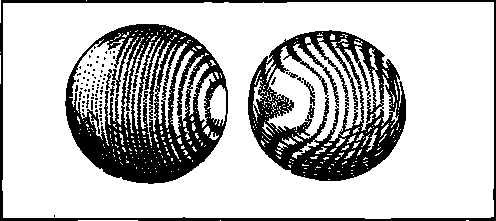
\includegraphics[width=0.8\textwidth]{figures/fig-02-06.pdf}
\caption{Finding defects using interference patterns.}
\label{fig-2.6}
\end{figure}

This method is widely used in optical work. For exam­ple, if we need to check the quality of the surface of a glass plate, this is done by considering the bands of equal thickness of a wedge of air set up by the plate with a perfect­ly smooth surface. If the two plates are pressed together at one end, a wedge of air is produced. If both surfaces are plane, the lines of equal thickness will be parallel lines.

Suppose the plate being tested has a depression or a bump. The lines of equal thickness will be bent because they bend around any defective spot. As the angle of incidence of light is changed, the bands move to one side or the other depending on whether the defect is a bump or a depression. \figr{fig-2.6} illustrates what the microscopic field looks like in such cases. Both patterns reveal defects in the samples. In the first case, the defect is located on the right edge, and in the other, it is on the left edge.

Exact measurements of refractive indices of a substance can be made with the aid of interference refractometers. These instruments reveal interference between two rays that have the largest possible separation.

Suppose in the path of one of the rays we have a body of length $l$ and refractive index $n$. If the refractive index of the medium is $n_{0}$, the optical difference of the path changes by $\Delta = l(n - n_{0})$. The two rays are brought to a single point by means of a focussing lens. What will we see in telescope? A system of light and dark bands. But these are not bands of equal thickness that can be seen with the unaided eye. The system of bands appearing in a refractometer is of a different origin. This is because the original beam of light is not ideally parallel but slightly divergent which means the light rays constituting the cone will fall on the plane at slightly different angles.

The interference events will occur in the same manner in the case of rays having the same inclination. And they will come together in the same spot of the focal plane of the telescope. If the path difference between the split portions of the beam changes, the bands will begin to move. If the path difference changes by the amount $\Delta$, then $\Delta /\lambda$ bands will pass through the eyepiece of the telescope.

The method is extremely precise because a displacement of 0.1 band can be detected with ease. For such a displace­ment, $\Delta = 0.1 \lambda = \SI{0.5d-5}{\centi\metre}$, and this permits detecting, over a length $l=\SI{10}{\centi\metre}$, a change in the refractive index amounting to \num{0.5d-6}.

We will now examine an interferometer of a different kind that does not utilize the phenomenon of refraction. This interferometer was made by the American physicist Albert Abraham Michelson (1852-1931). It is hard to overestimate the role this instrument played in the histo­ry of physics (I make bold to say, even the history of human thought). Through the use of this interferometer, a fact of exceptional importance was discovered: the speed of light in directions along the earth’s orbit and across it is the same.

What this means is that the speed of light does not depend on the motion of the light source! This means that the speed of light is not combined with the speed of motion of the lamp (that produces the light flash) in accord with the rules by which the speed of a bullet is combined with the speed of the man holding the gun. The discovery of this remarkable fact led to the theory of relativity and to a fundamental reconsideration of the meaning of such basic scientific concepts as length, time, mass, and energy. We will go into these important mat­ters later on. The \emph{Michelson interferometer} is of interest not only because of the place it occupies in the history of physics but also because the simple principles under­ lying its construction are still used today to measure lengths and distances.

\begin{figure}[!ht]
\centering
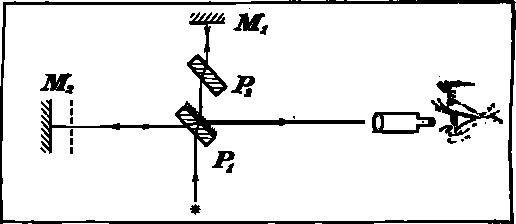
\includegraphics[width=0.8\textwidth]{figures/fig-02-07.pdf}
\caption{The Michelson interferometer.}
\label{fig-2.7}
\end{figure}

In this instrument, a parallel beam of monochromatic light falls on a plane-parallel plate $P_{1}$ (\figr{fig-2.7}) cov­ered with a translucent layer of silver on the ruled side. This plate is placed at an angle of \ang{45} to the light ray falling from the source and splits it in two, one ray moving parallel to the incident ray (to mirror $M_{1}$) and the other perpendicular to mirror $M_{2}$. The separated rays of light fall on the two mirrors at zero angles of incidence and return to the very same spots of the translucent plate from which they emerged. Each ray returning from the mirror is again split on the plate. Part of the light returns to the source and the other part enters the telescope. In the figure you can see that the ray coming from the mirror opposite the telescope passes twice through the glass plate with its translucent layer. For this reason, in order to ensure equality of the optical paths, the ray coming from mirror $M_{1}$ is passed through a compensating plate $P_{2}$ that is identical to the first plate but without the translucent layer.

In the field of view of the telescope, circular rings are observed that correspond to interference in the layer of air (the thickness of which is equal to the difference between the distances of the mirrors from the site of beam-splitting) of the primary rays forming the cone. A displacement of one of the mirrors (for instance, $M_{2}$ to the position shown by the dashed line) by a fourth of a wavelength will correspond to a transition from maxi­mum to minimum, that is, it will cause a shift in the pattern through half a circle. This can be clearly detected by an observer. Thus, in violet rays the sensitivity of an interferometer is better than \SI{1000}{\angstrom} (angstroms).

The advent of lasers produced a revolution in the technique of interferometry.

Did you ever wonder why an interference rainbow ap­pears on films of oil floating on water but does not appear in window glass? The situation would seem to be quite similar: in both cases, rays are reflected from an outer and an inner surface of a plate. In both cases, the two reflected rays combine. But interference is observed only when the plate is thin. I’ve used this question at exami­nations and confused many a student.

The essence of the matter is this. The emission time of an atom is equal to \num{d-8}or \num{d-9} second. The single act of emission consists in the release of a wave train. Since the time of emission is very small, the wave train is very short despite the great velocity of light. When we split a ray into parts, only two parts of the same wave train can undergo interference. This means that one portion of the sine curve must appreciably overlap another por­tion. But for this to happen, it is naturally necessary that the path difference between the split portions of the ray be substantially less than the length of the wave train. The condition is met in the case of a micron-thin film, but not in the case of window glass. That is the answer the student should have given.

The maximum path difference between the rays when interference can be observed is termed the \emph{coherence length}. For light, this amounts to a fraction of a millimetre.

Now notice how radically the situation changes in the case of laser emission. A continuous-action laser creates photons of stimulated emission that set out in the same phase. Or, to use wave language, the wave trains ema­nating from different atoms are superimposed on one another thus creating what appears to be a single wave. The coherence length becomes practically unbounded; at any rate, it is measured in metres and kilometres (as is always the case, the ideal is never attainable but I will not dwell here on the variety of factors that affect the coherence length).


Using laser light, it is possible to construct interfer­ometers capable of handling problems that until recently had appeared unsolvable. For example, using an ordinary light source, the mirror in the Michelson interferometer can be displaced only distances of the order of a millimetre. Now if the light ray is produced by a laser, the path of the ray falling on mirror $M_{1}$ may be made equal to several centimetres and the path of the ray reflected from mirror $M_{2}$, tens of metres.


Interferometers to check the sphericity of lenses can be made with a single surface of comparison whereas, if we use ordinary light, one has to change the standard of comparison along with any change in the radius of the lens being tested (this is because one cannot work with large path differences). Which is to say nothing about the fact that the interference patterns have become incomparably brighter and for that reason can be analyzed more easily and exactly.

The possibility of getting along without compensation of the optical path of one of the rays makes it possible to design interferometers of an entirely new type. It has now become possible to detect displacements of dams, geological drift, oscillations of the earth’s crust. By re­flecting laser light from objects located at large distances and then making it interfere with the original light, we can carry out exact measurements of the speed of motion of such objects.

\section{Laser Devices}

A device that produces a laser beam can of course be called an instrument because it is used for analysis, control, and observations. However, unlike other optical instruments, the laser plays a far greater role in industry. The use of lasers is so widespread that we will again and again come back to them. In this section we will discuss the use of lasers in working various materials. If it is not high power that is required, use can be made of the compact neodymium laser. The heart of this laser is, as we have already mentioned, glass alloyed with neody­mium. A glass rod 50 millimetres long and 4 millimetres in diameter. The light flash that does the pumping is given by a xenon lamp. In order to cut losses of luminous energy, the lamp and rod are enclosed in a water-cooled cylindrical chamber.

The following properties are important in the use of this type of instrument and its analogues: the possibility of localizing energy over an extremely small area, the possibility of precise batching of portions of energy, and the possibility of delivering energy without the use of any wires or contacts.

Take the use of lasers in the watch industry. A watch requires jewels. These are often in the form of rubies; the more rubies the higher the quality of the watch. Apertures have to be drilled in tiny ruby discs. Ordinarily, without lasers, this operation takes several minutes for each jewel. Using lasers, the process is completely automatic and takes a fraction of a second. And since industry uses many millions of these a year, the obvious gain in time is tremendous.

The laser is extremely important also in the diamond industry. Drilling and broaching of diamonds is easily handled by lasers which can make a diamond into any shape or produce apertures as small as a few micrometres.

But let’s get back to watches. A laser can weld the spring to the watch mechanism. Quite obviously, wher­ever high-precision welding is required -- and this is the order of the day in many areas of high-precision technol­ogy -- laser beams are employed with excellent results. The great advantage of this needle-thin ray is that there is no need to protect and cool adjacent parts of the com­ponent being welded.

Lasers are of course used trivially as a knife to cut out any imaginable patterns on any kind of material. Lasers have invaded some rare professions as well. Take the restoration of marble sculptures. The atmosphere of the twentieth century is unfortunately quite pollut­ed. A great variety of noxious gases, particularly sulphur oxide, form a black crust on marble. This crust is porous and acts as a sponge packing up more moisture and more harmful substances. Removing the crust by mechanical or chemical means can often ruin the sculpture. Now a laser operating in a pulsed regime can remove the crust without harming the underlying marble.

A carbon dioxide laser can be used to grow crystals without resorting to the crucible. This is not a new pro­cedure. High-frequency currents have long been used in this capacity, but not for dielectric materials that possess too low a thermal conductivity. Today, lasers are used to grow crystals (without using crucibles) of niobates and other much needed materials. The importance of the non-crucible growth of crystals for the needs of microelec­tronics cannot be overestimated because even a few parts in a million of impurities can play a negative role, and in a crucible it is practically impossible to keep harmful atoms from passing from the material of the crucible into the crystal.

I will not describe the apparatus used in such cases. Crystal growth was discussed in the second book of our series. As in the case of high-frequency currents, the laser beam creates a small molten zone that slowly brings the material up to the growing crystal. I think it very prob­able that lasers will be supplanting other methods of crystal growth as well.

\section{Photometry}
Every source of light may be characterized by the energy it emits. However, in many cases we are only interested in that part of the energy flux that produces a visual sensation. As we have already mentioned, this is characteristic of electromagnetic waves of wavelength between roughly 380 and 780 nanometres.

Light perceived by our brain is characterized by lumi­nance (brightness) and colour. If we compare the visual sensations created by light of equal intensity but different wavelength, it will be apparent that the eye perceives as brightest light that has a wavelength of 555 nanome­tres. This is green.

The perception of light is shown as a \emph{visibility} (or \emph{luminosity}) \emph{curve} in \figr{fig-2.8}, which represents (in relative units) the sensitivity of the normal human eye to waves of different length. However, engineers disre­gard this curve and leave it up to the human eye to judge the integral \emph{luminous intensity}. The first thing, in that case, is to choose a standard light source and then compare other sources with the standard. For a long time, the unit of luminous intensity was the \emph{candle} because at first attempts were made to find a certain standard candle flame. It is quite obvious that this is no easy job.

\begin{figure}[!ht]
\centering
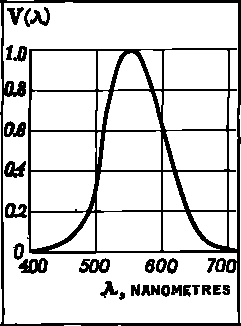
\includegraphics[width=0.4\textwidth]{figures/fig-02-08.pdf}
\caption{Sensitivity of human eye to different wavelengths shown in a \emph{visibility curve}.}
\label{fig-2.8}
\end{figure}
The international standard today is an incandescent black body. The material is platinum. The black body emits light radiated through a small aperture by plati­num heated to the melting point, or \SI{1769}{\celsius}.

The unit of luminous intensity is the \emph{candela} (which is Latin for ``candle''). The international definition avoids any direct indication as to temperature of luminescence (this is done to avoid errors associated with measuring the temperature). The candela is defined thus: if we take, as the source, platinum as it solidifies at normal atmospheric pressure, then an area of $(1/6)\SI{d-5}{\meter\squared}$ yields a luminous intensity, in the direction perpendicular to the surface, equal to one candela.

The definition of luminous intensity and its unit are surprisingly archaic. Specialists realize this and they hope that in the near future a new basis will be chosen: energy measurements and the standard luminosity curve. Then luminous intensity can be defined by multiplying these two spectral distributions. If we multiply these two func­tions and integrate the product, we obtain a measure of luminous intensity. For the reader who is not acquainted with integral calculus I can restate this as follows: multiply the intensities of the separate spectral portions by their luminosity factors and then combine all the products.

At sufficiently large distances, a light source appears as a point. That is just when it is convenient to measure luminous intensity. Now, around this point source let us construct a sphere and on the surface of the sphere a portion of area $S$. Dividing $S$ by the square of the dis­tance from the centre, we obtain the so-called solid angle. The unit of the solid angle is the steradian. If we cut out an area $S= 1$ square metre on a sphere of radius one metre, the solid angle is equal to one 
steradian.

\emph{Luminous flux} is the luminous intensity of a point source multiplied by the solid angle.

Do not be upset by the fact that the luminous flux becomes zero (vanishes) when we speak of parallel rays. That is because the concept of luminous flux is not used in such cases.

The unit of luminous flux is the \emph{lumen}, which is equal to the flux delivered by a point source with a luminous intensity of one candela to an angle equal to one steradian. The overall (total) luminous flux emitted by a point in all directions is equal to $4\pi$ lumens.

Luminous intensity characterizes a light source irre­spective of its surface. Yet it is quite obvious that the impression will differ depending on the extent of the source.
For this reason, use is made of the notion of \emph{luminance} (\emph{brightness}) of a source. This is the luminous intensity per unit surface of the light source. Luminance is mea­sured in \emph{stilbs}: one stilb is equal to one candela per square centimetre.

One and the same light source brings different luminous energy to the page of an open book depending on where the source is located. What is important to the reader is the illumination of the portion of his desk in which his book lies. \emph{Illumination} is defined as the luminous intensi­ty divided by the square of the distance from the point source. Why the square? Because a luminous flux remains unchanged inside a given solid angle, no matter how far we recede from the glowing point. Now, the area of the sphere and the area of the portion cut out by the solid angle will increase in inverse proportion to the square of the distance. This simple rule is called the \emph{inverse-square law}. If the distance of the book from a small lamp is increased from 1 metre to 10 metres, we thus reduce the illumination of the page by a factor of one hundred. 

The \emph{lux} is the unit of illumination. This is the illumi­nation generated by a luminous flux equal to one lumen over an area of one square metre.

The illumination on a moonless night is equal to \SI{0.0003}{\lux}. On a night with full moon the illumination can reach \SI{0.2}{\lux}. For comfortable reading we need an illu­mination of \SI{30}{\lux}. When shooting movie scenes, powerful projectors are used that raise the illumination to \SI{10000}{\lux}.

So far we have not mentioned the instruments that measure luminous fluxes and illumination. At the present time, such measurements are no problem. Actually, we proceed exactly as we did in providing the new definition of the candela. We measure the energy falling on a pho­tocell and graduate the scale of the photocell in units
of lux with account taken of the luminosity curve.

Photometers in use last century operated on the prin­ciple of comparing the luminances (brightnesses) of two adjoining illuminated areas. One area received light that was to be measured; on the other, using simple devices, one reduced the luminous flux a known number of times until the two adjoining areas had the same illumination.

\section{Holography}

The invention of lasers has opened up a new chapter in the development of science and technology. It is hard to find a branch of knowledge in which stimulated emis­sion has not revealed fresh vistas.

In 1947, Dennis Gabor (1900-1979) outlined the principles of obtaining images of objects in a radically different way from photography. The new technique is called \emph{holo­graphy}. Holography became possible because of the pe­culiarities of stimulated emission that make it different from ordinary light. Let us stress once again that in laser radiation nearly all photons coincide in all their features: frequency, phase, polarization, and direction of propagation. A laser beam is hardly at all spread out, which means an extremely narrow beam can be thrown to great distances from the source; laser beams have the property of a very great coherence length. It is due to this circumstance (which is particularly important in holography) that interference of split rays with a large path difference is possible.

\begin{figure}[!ht]
\centering
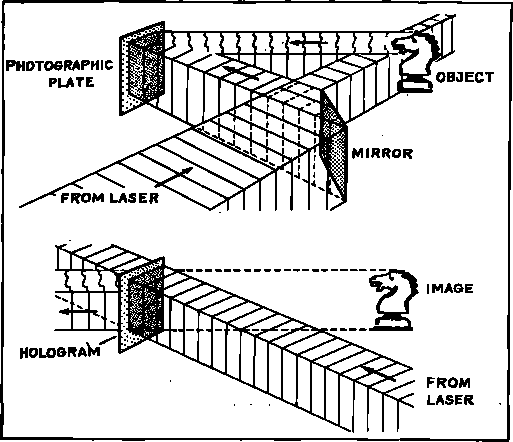
\includegraphics[width=0.9\textwidth]{figures/fig-02-09.pdf}
\caption{Technique of creating a hologram.}
\label{fig-2.9}
\end{figure}
The upper part of \figr{fig-2.9} illustrates the technique of obtaining a hologram. The object of interest is illum­inated with a broad and weak (so as not to harm the object) laser beam. The same beam is scattered by the object and by a mirror, which generates a so-called refer­ence wave. The two waves are superimposed, interference occurs, and the pattern is recorded on a photographic plate.
\begin{figure}[!ht]
\centering
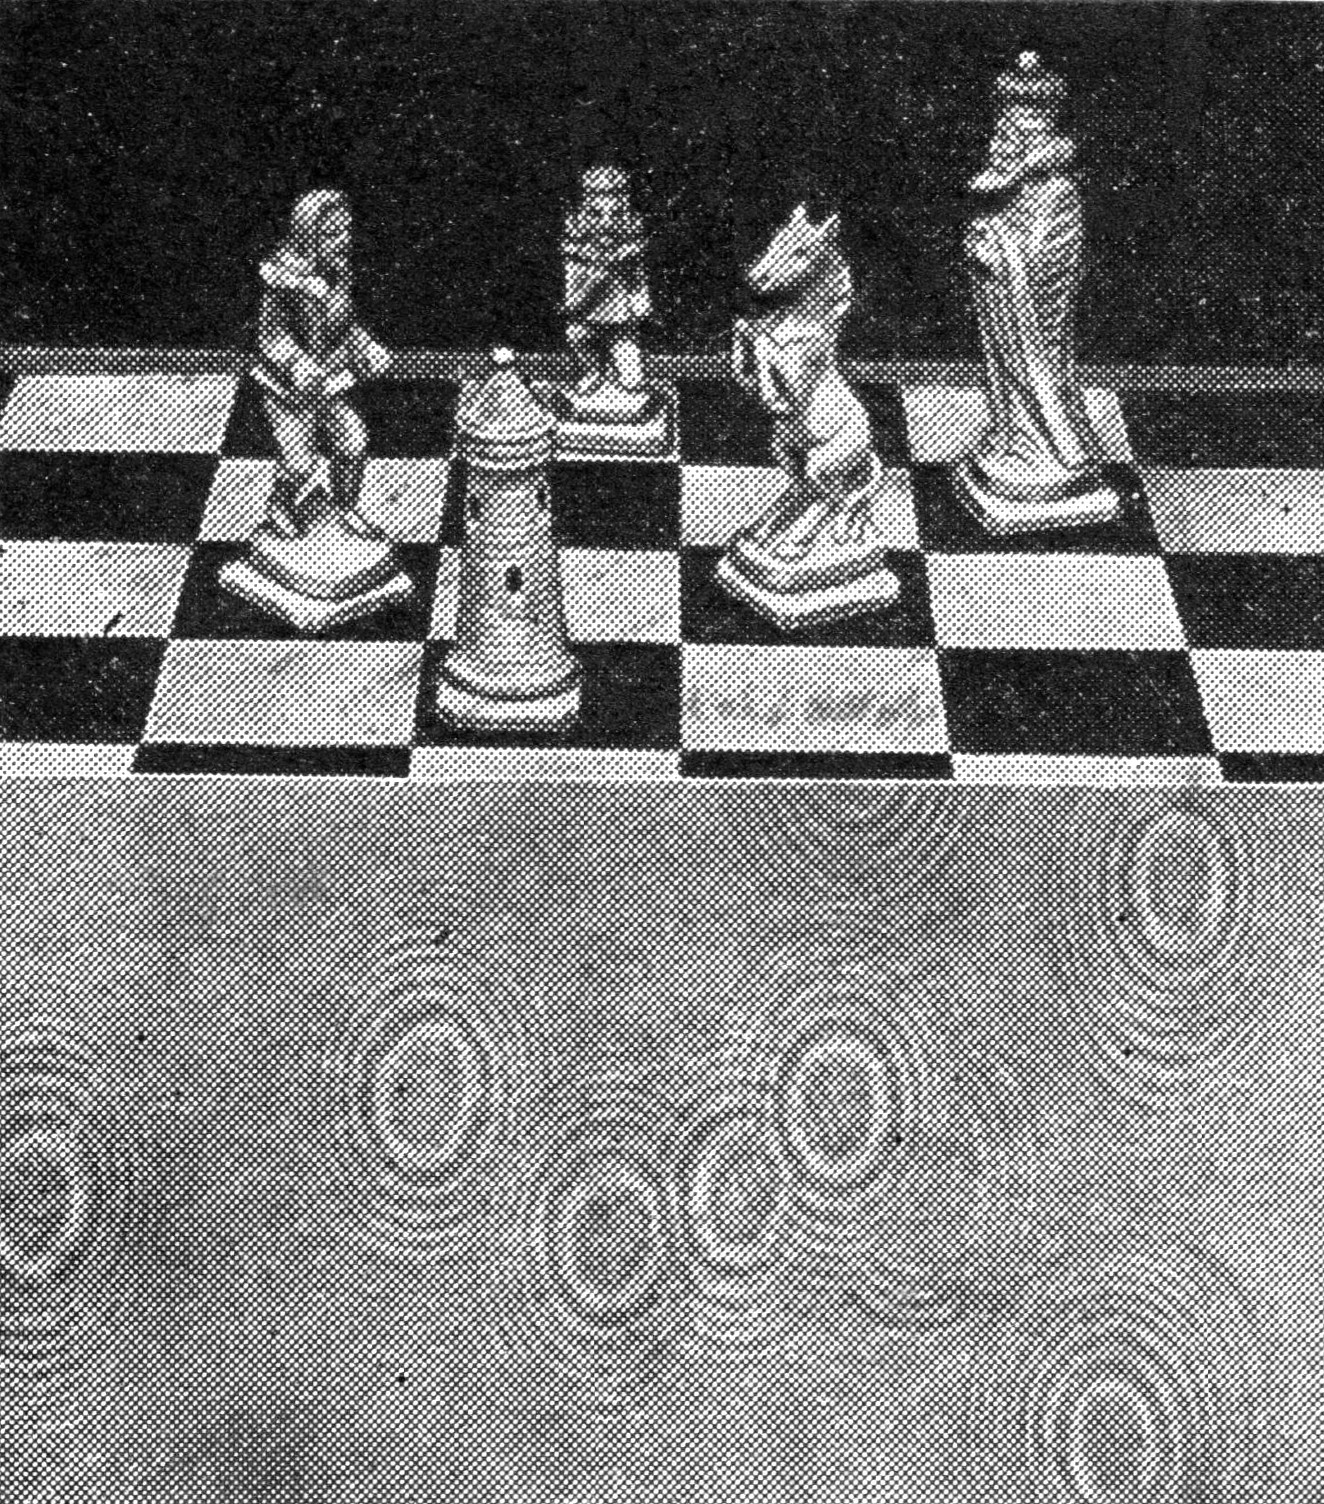
\includegraphics[width=0.6\textwidth]{figures/fig-02-10.jpg}
\caption{The object and its hologram.}
\label{fig-2.10}
\end{figure}
Take a look at \figr{fig-2.10}. The object is shown above, the ``image'' below. Yes, this is the image. It is an intri­cate combination of dark and light rings called a hologram and is indeed the image of the object, only it is a latent (hidden) image. The hologram contains complete infor­mation about the object; it would be more correct to say complete information about the electromagnetic wave scattered by the chess pieces. A photograph does not contain so much information. The best photograph conveys precisely all information about the intensity of the scattered rays. But a wave scattered by any point of an object is fully characterized not only by its intensity (amplitude) but also by its phase. A hologram is an in­terference pattern and each light or dark line describes not only the intensity but also the phase of the rays coming from the object onto the appropriate spots of the photographic plate.

A hologram, like any ordinary photographic plate, can be developed, fixed, and stored for any length of time. Whenever we want to, we can view the object by irra­diating the hologram, as shown in the lower part of \figr{fig-2.9}, with light from the same laser, thus reconstructing the original geometric arrangement: the laser beam is directed like the beam reflected from mirror. Then an image of the object appears where the object once stood, and that image, ideally, is identical to the picture that confronted the eye.

We will not go into the theory of obtaining holograms. The basic idea is that when a hologram is illuminated, there arise scattered waves with the same amplitudes
and phases as those that created the hologram originally. These waves combine to form a wave front that is identi­cal to the wave front that produced the hologram. What occurs is a peculiar reconstruction of the wave when the hologram is illuminated in the same conditions that the object was illuminated. The result is an image of the object.

Research in the field of holography continues. We are now able to obtain coloured images. Improved results are possible by taking several holograms from different angles. Finally (and this is perhaps the most important thing) it turns out that we can examine holograms without resorting to lasers.

There are books which treat the subject of holography in detail. Holography merits our attention for the reason that it is high-capacity method for storing three-dimen­sional information concerning an object. Future research will undoubtedly bring holography into new fields of technology and into the home.


%
%%\newpage
%\begin{center}
%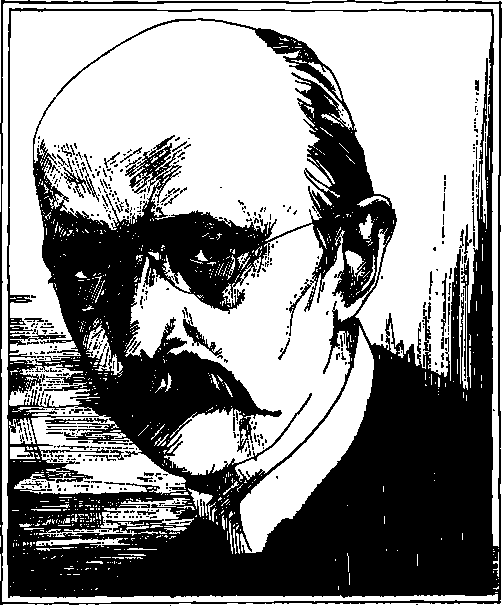
\includegraphics[width=\textwidth]{figures/planck.pdf}
%\end{center}
%{\small \textsf{\hlred{Max Planck [1858-1947]}} -- \textsf{\footnotesize outstanding German scientist who laid the foundations of quantum theory. In an attempt to find a mathematical expression for a proper description of the spectral distribution of the emission of an ideal black body Planck demonstrated that such a formula could be obtained by introducing a ``quantum of action''. Planck assumed that a body emits energy in parcels, equal to the product of a constant (which later was named after him) by the frequency of the light.}}



